\documentclass[aspectratio=169]{beamer}
\usefonttheme[onlymath]{serif}
\usepackage[brazilian]{babel}

\mode<presentation>
{
  \usetheme{Darmstadt}     % or try Darmstadt, Madrid, Warsaw, ...
  \usecolortheme{beaver} % or try albatross, beaver, crane, ...
  \usefonttheme{default}  % or try serif, structurebold, ...
  \setbeamertemplate{navigation symbols}{}
  \setbeamertemplate{caption}[numbered]
  \setbeamertemplate{headline}{}
}

%%%%%%%%%%%%%%%%%%%%%%%%%%%%%%%%%%%%%%%%%%%%%%%%%%%%%%%%%

\usepackage{mathtools}
%\usepackage{amsthm}
\usepackage{amsmath}
%\usepackage{nccmath}
\usepackage{amssymb}
%\usepackage{amsfonts}
\usepackage{physics}
%\usepackage{dsfont}
%\usepackage{mathrsfs}
%\usepackage{slashed}    % Feynman slash notation, requires LuaLaTeX
%\usepackage[compat=1.1.0]{tikz-feynman}   % Feynman diagrams

%\usepackage{titling}
\usepackage{indentfirst}
%\usepackage[titletoc,title]{appendix}
%\renewcommand\appendixname{Apêndice}

\usepackage{bm}
%\usepackage{xcolor}
%\usepackage[dvipsnames]{xcolor}
\usepackage{cancel}

%\usepackage{xurl}
\usepackage{hyperref}
\usepackage{cite}

\usepackage{float}
\usepackage{graphicx}
\usepackage{tikz}
\usepackage{caption}
\usepackage{subcaption}

%%%%%%%%%%%%%%%%%%%%%%%%%%%%%%%%%%%%%%%%%%%%%%%%%%%

\newcommand{\eps}{\epsilon}
\newcommand{\vphi}{\varphi}
\newcommand{\cte}{\text{cte}}

\newcommand{\N}{\mathbb{N}}
\newcommand{\Z}{\mathbb{Z}}
\newcommand{\Q}{\mathbb{Q}}
\newcommand{\R}{\mathbb{R}}
\newcommand{\C}{\mathbb{C}}
\renewcommand{\P}{\mathbb{P}}
\renewcommand{\H}{\s{H}}

\newcommand{\0}{\vb{0}}
\newcommand{\1}{\mathds{1}}
\newcommand{\E}{\vb{E}}
\newcommand{\B}{\vb{B}}
\renewcommand{\v}{\vb{v}}
\renewcommand{\r}{\vb{r}}
\newcommand{\p}{\vb{p}}
\newcommand{\q}{\vb{q}}
\newcommand{\F}{\vb{F}}
\newcommand{\dtcp}{\delta_{\text{CP}}}

\newcommand{\s}[1]{\mathcal{#1}}
\renewcommand{\sl}[1]{\slashed{#1}}
\newcommand{\prodint}[2]{\left\langle #1 , #2 \right\rangle}
\newcommand{\cc}[1]{\overline{#1}}
\newcommand{\Eval}[3]{\eval{\left( #1 \right)}_{#2}^{#3}}

\newcommand{\unit}[1]{\; \mathrm{#1}}

\newcommand{\n}{\medskip}
\newcommand{\e}{\quad \mathrm{e} \quad}
\newcommand{\ou}{\quad \mathrm{ou} \quad}
\newcommand{\virg}{\, , \;}
\newcommand{\ptodo}{\forall \,}
\newcommand{\existe}{\exists \,}
\renewcommand{\implies}{\; \Rightarrow \;}
%\newcommand{\eqname}[1]{\tag*{#1}} % Tag equation with name

% MACROS
\newcommand{\dcp}{\delta_{\text{CP}}}


%%%%%%%%%%%%%%%%%%%%%%%%%%%%%%%%%%%%%%%%%%%%%%%%%%%%%%%%%

\title[Física de Neutrinos na Física de Partículas Elementares]{\LARGE{Física de Neutrinos na Física de Partículas Elementares}}
\author[Mateus Marques]{\large{Mateus Marques}\\[2ex]\small{Orientadora: Renata Zukanovich Funchal}}
\institute[]{\small{Instituto de Física da Universidade de São Paulo}}
\date[SIICUSP 30, 2022]{\small{SIICUSP 30, 2022}}
\titlegraphic{
\includegraphics[height=1.5cm]{logos/ifusp.png}}

\begin{document}

\begin{frame}
  \titlepage
\end{frame}

\section{Introdução}

\begin{frame}{Introdução}

\begin{itemize}
%
\item Neutrinos interagem \textit{muito fracamente} com a matéria. Eles foram previstos por Wolfgang Pauli em 1930 como partículas extras no decaimento $\beta$
\begin{equation} \label{eq:beta}
n^0 \to p^+ + e^- + \cc{\nu_e}.
\end{equation}

\item Neutrinos solares foram detectados pela primeira vez em 1968 pelo experimento Homestake, que mediu um fluxo de neutrinos próximo de um terço do previsto teoricamente pelo Modelo Padrão Solar. Essa discrepância ficou conhecida como \textit{problema do neutrino solar}.

\item Essa foi uma forte evidência para o fenômeno de oscilação de neutrinos, que estabelece que os neutrinos têm massa não-nula. Em 2002 e 2015, quatro físicos receberam o prêmio Nobel por contribuirem em experimentos sobre neutrinos solares e oscilações de neutrinos.

\item O Modelo Padrão da Física de Partículas prevê que os neutrinos têm massa nula \cite{gonzalez}. Assim, o fenômeno de oscilação de neutrinos é um grande indício de existência de física além do Modelo Padrão.

%
\end{itemize}


%\vskip 1cm
%\begin{block}{Examples}
%$n=3$.
%\end{block}

\end{frame}

\section{Oscilação de Neutrinos}

\begin{frame}{Oscilação de Neutrinos}

O ponto de partida na fenomenologia das oscilações de neutrinos é que estes interagem apenas em seus autoestados de sabor $\nu_e, \nu_\mu$ e $\nu_\tau$ (associados aos léptons $e^-$, $\mu^-$ e $\tau^-$), porém evoluem no tempo por uma hamiltoniana $H$ que possui outros autoestados (de massa) $\nu_1, \nu_2$ e $\nu_3$.

\n

No vácuo, a energia dos neutrinos vem da expressão relativística:
\begin{equation} \label{eq:aprox-energ}
E_i = \sqrt{p^2 + m_i^2} \approx
p \qty( 1 + \frac{m_i^2}{2 p^2} ) \approx
E + \frac{m_i^2}{2E}.
\end{equation}

Por $H \ket{\nu_i} = E_i \ket{\nu_i}$ e pela matriz de mistura leptônica $U$ \cite{gonzalez} entre as bases de sabor e de massa, $\ket{\nu_\alpha} = \sum_j U_{\alpha j} \ket{\nu_j}$, temos a equação de Schrödinger
\begin{equation} \label{eq:3nu-vacuo}
i \dv{t}
\begin{pmatrix}
\psi_e \\ \psi_\mu \\ \psi_\tau
\end{pmatrix}
=
\qty[ \frac{1}{2E} \, U
\begin{pmatrix}
0 & 0 & 0 \\
0 & \Delta m_{21}^2 & 0 \\
0 & 0 & \Delta m_{31}^2 \\
\end{pmatrix}
\, U^\dagger ]
\begin{pmatrix}
\psi_e \\ \psi_\mu \\ \psi_\tau
\end{pmatrix}.
\end{equation}

\end{frame}

\begin{frame}{Oscilação de Neutrinos no Vácuo}

\begin{figure}[H]
\centering
\begin{subfigure}{.48\textwidth}
  \centering
  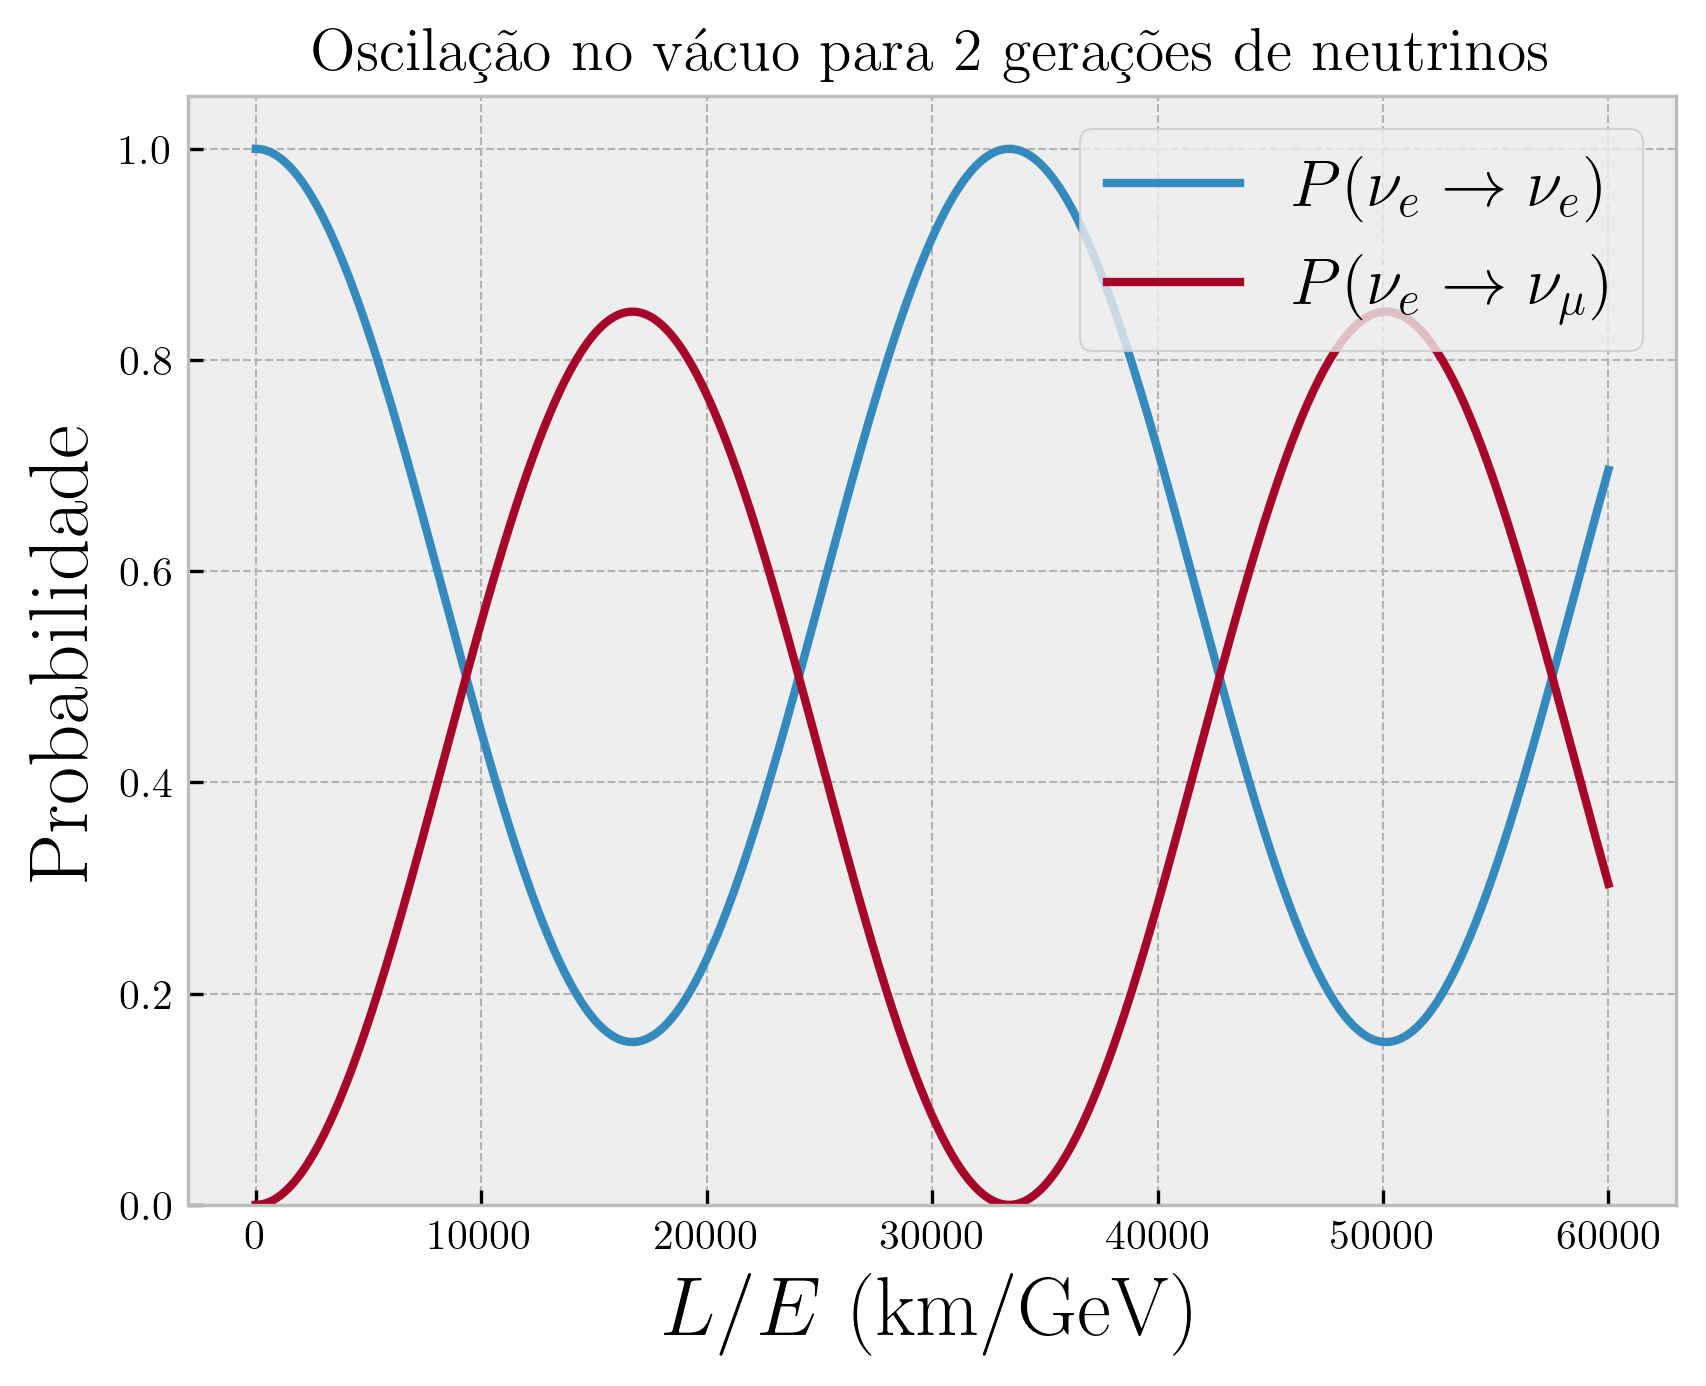
\includegraphics[width=\linewidth]{fig/2nu-vacuo-e.png}
  \label{fig:2nu-vacuo-e}
\end{subfigure}%
\quad
\begin{subfigure}{.48\textwidth}
  \centering
  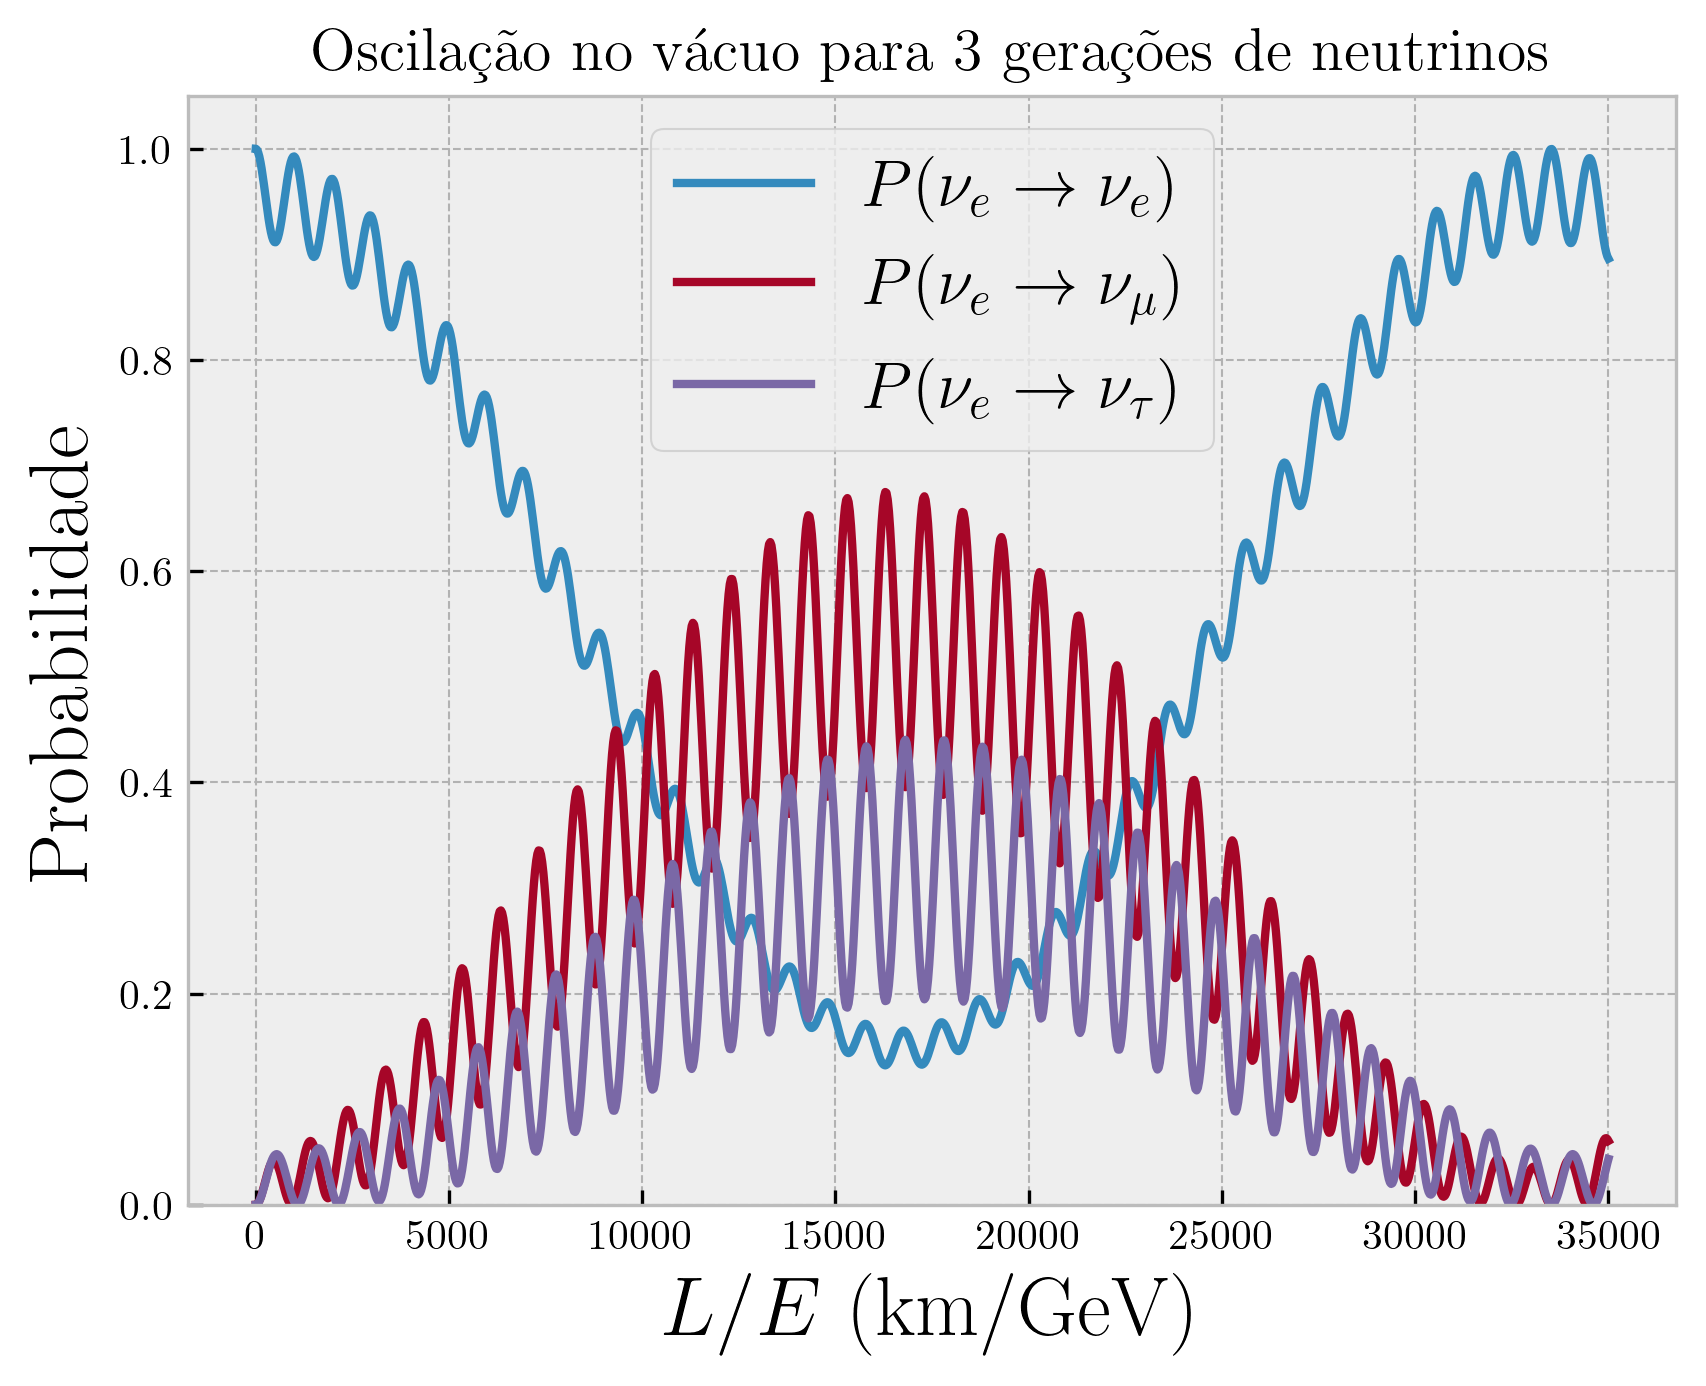
\includegraphics[width=\linewidth]{fig/3nu-vacuo-e.png}
  \label{fig:3nu-vacuo-e}
\end{subfigure}
\caption{Oscilação de um neutrino $\nu_e$ no vácuo com os parâmetros do NuFIT \cite{nufit}. $\Delta m_{21}^2 = 7.42 \times 10^{-5} \unit{eV^2}$, $\Delta m_{31}^2 = 2.515 \times 10^{-3} \unit{eV^2}$, $\theta_{12} = 33.44^\circ$ e $\theta_{13} = 8.57^\circ$.}
\label{fig:vacuo_electron}
\end{figure}

\end{frame}

\section{Oscilação na Matéria}

\begin{frame}{Oscilação no Sol}

No Modelo Padrão, o neutrino interage apenas através da força fraca, que é intermediada pelos bósons vetoriais $W^\pm$ e $Z^0$. O propagador deles é dado por \cite{halzen}
\begin{equation} \label{eq:boson-propagator}
\frac{i (- g^{\mu \nu} + p^{\mu} p^{\nu} / M^2)}{p^2 - M^2}.
\end{equation}

Como a massa desses bósons é da ordem de $M \sim 100 \unit{GeV}$, temos que $p^2 \ll M^2$ e o propagador se reduz essencialmente a uma constante $G_F$ (de Fermi).

\n

Quando neutrinos propagam na matéria, podemos ter espalhamentos coerentes ou incoerentes. Para espalhamentos incoerentes, a seção de choque é muito baixa \cite{gonzalez}. A corrente neutra (intermediada por $Z^0$) apenas contribui com um fase global, igual para todos os neutrinos \cite{gonzalez}.

\n

Nos concentrando então em espalhamentos coerentes de corrente carregada, chegamos ao potencial efetivo de baixas energias e dependente do tempo
\begin{equation} \label{eq:eff-pot}
V(t) = \sqrt{2} \, G_F N_e(t) \cdot \text{diag}(1, 0, 0),
\end{equation}
onde $N_e$ é a densidade eletrônica no interior do Sol.

\end{frame}

\section{Resultados}

\begin{frame}{Abordagem Numérica}

Para resolvermos a equação de evolução dos neutrinos no interior do Sol, recorremos ao método de integração geométrico denominado \textit{expansão Magnus} \cite{efficient}.

\n

A expansão Magnus consiste na representação exponencial (série de Dyson) da solução da equação de Schrödinger:
\begin{equation} \label{eq:schrodinger}
i \dv{\Psi}{t} = H \Psi \implies \Psi(t) = e^{-i \Omega(t, t_0)} \Psi_0,
\end{equation}
onde $\Omega(t, t_0) = \sum_{k=1}^\infty \Omega_k(t, t_0)$ e cada $\Omega_k$ é dado por múltiplas integrais envolvendo comutadores de $H(t)$ (temporalmente ordenados pelo operador $\s{T}$).

\n

A ideia então é aplicar iterações
\begin{equation} \label{eq:magnus}
\Psi(t_{n+1}) = e^{-i \Omega^{(p)}(t_n + h_n, t_n)} \Psi(t_n),
\end{equation}
onde truncamos $\Omega^{(p)}(t_n + h_n, t_n) = \sum_{k=1}^p \Omega_k(t_n + h_n, t_n)$ em $p = m - 2$, sendo $m + 1$ a ordem do erro de $\Psi(t_n)$ em cada iteração.
\end{frame}


\begin{frame}{Resultados}

Utilizamos os dados do modelo solar \texttt{BS2005} \cite{bahcall}. Interpolamos a densidade eletrônica $N_e$ e tomamos as médias no ponto de produção de neutrinos para diferentes mecanismos de reação no interior do Sol.

\begin{figure}[H]
\centering
\begin{subfigure}{.5\textwidth}
  \centering
  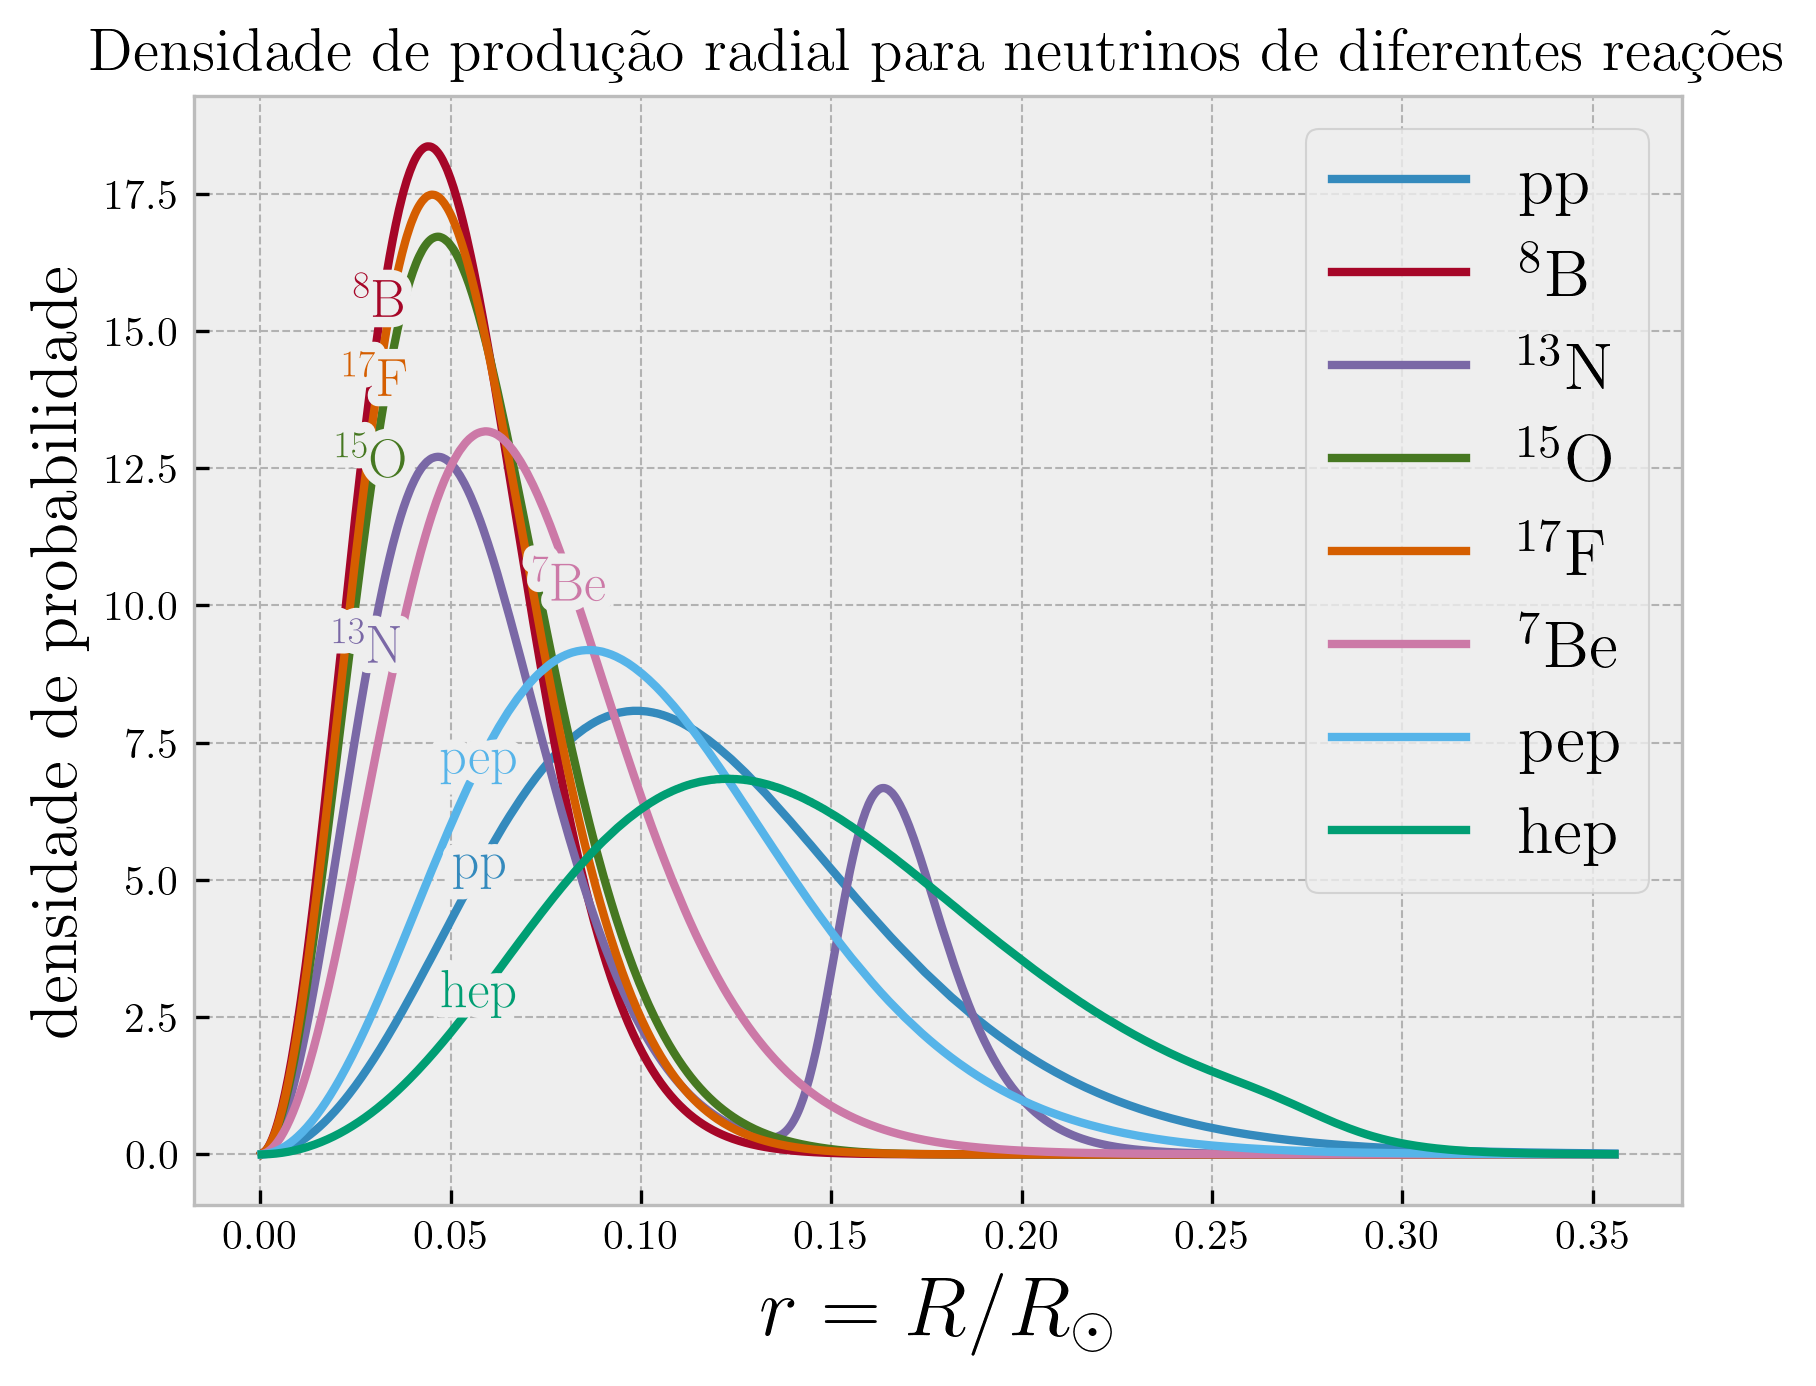
\includegraphics[width=0.89\linewidth]{fig/raio.png}
  \label{fig:raio}
\end{subfigure}%
\begin{subfigure}{.5\textwidth}
  \centering
  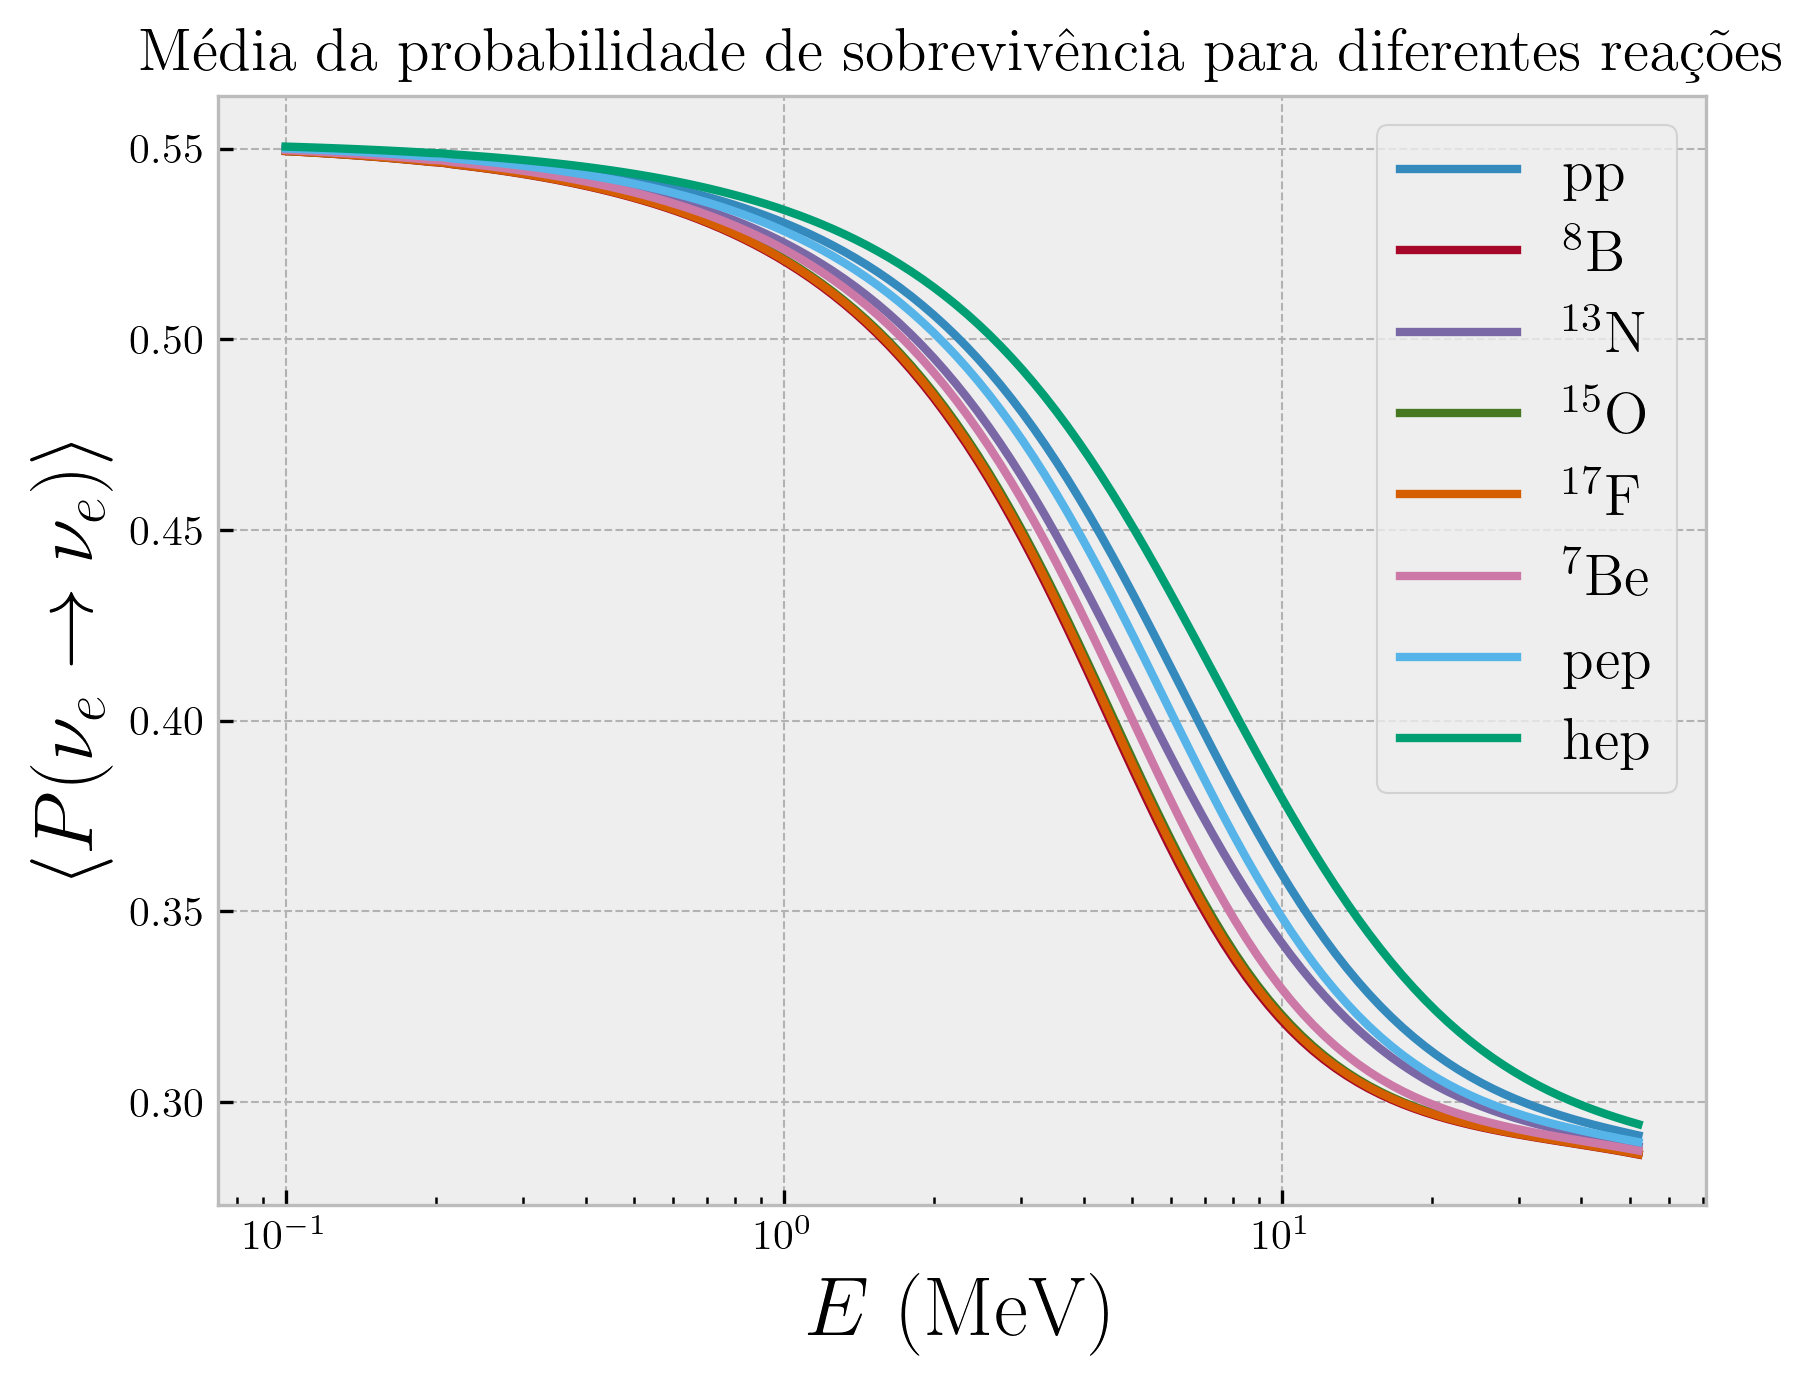
\includegraphics[width=0.89\linewidth]{fig/surv_prob.png}
  \label{fig:surv_prob}
\end{subfigure}
\caption{Densidades de produção radial de neutrinos e suas respectivas probabilidades médias de sobrevivência $\ev{P(\nu_e \to \nu_e)}$ ao sair do Sol como função da energia $E$.}
\label{fig:resultados}
\end{figure}

\end{frame}


\section{Referências}

\begin{frame}{Referências}

\footnotesize

\begin{thebibliography}{10}
\bibitem{gonzalez}
\alert{M. C. Gonzalez-Garcia, Y. Nir.}
\newblock {Neutrino masses and mixing: evidence and implications.}
\newblock {\textit{Rev. Mod. Phys.}, vol. 75, pp. 345-402, Mar 2003.}

\bibitem{nufit}
\alert{NuFIT Collaboration.}
\newblock {NuFIT website. Data from October 2021.}
\newblock {\url{http://www.nu-fit.org}.}

\bibitem{halzen}
\alert{F. Halzen, A. D. Martin.}
\newblock {Quarks \& Leptons: An Introductory Course In Modern Particle Physics.}
\newblock {John Wiley \& Sons, 2008.}

\bibitem{efficient}
\alert{F. Casas, J. C. D'Olivo, J. A. Oteo.}
\newblock {Efficient numerical integration of neutrino oscillations in matter.}
\newblock {\textit{Phys. Rev. D}, vol. 94, p. 113008, Dec 2016.}

\bibitem{bahcall}
\alert{J. N. Bahcall.}
\newblock {John Bahcall's website.}
\newblock {\url{http://www.sns.ias.edu/~jnb}.}

\end{thebibliography}

\end{frame}


\section{Agradecimentos}

\begin{frame}{Agradecimentos}

\begin{figure}[H]
\centering
\begin{subfigure}{.3\textwidth}
  \centering
  
\includegraphics[width=0.6\linewidth]{logos/siicusp30.png}
  \label{logo:siicusp}
\end{subfigure}
\begin{subfigure}{.3\textwidth}
  \centering
  
\includegraphics[width=0.6\linewidth]{logos/usp.jpg}
  \label{logo:usp}
\end{subfigure}
\end{figure}

\n\n

\begin{figure}[H]
\centering
\begin{subfigure}{.3\textwidth}
  \centering
  
\includegraphics[width=0.8\linewidth]{logos/ifusp.png}
  \label{logo:ifusp}
\end{subfigure}
\begin{subfigure}{.3\textwidth}
  \centering
  
\includegraphics[width=0.8\linewidth]{logos/fapesp.png}
  \label{logo:fapesp}
\end{subfigure}
\end{figure}

%\begin{figure}
%    \centering
%    
\includegraphics[width=3cm]{logos/ifusp.png}
%\end{figure}
%
%\begin{figure}
%    \centering
%    
\includegraphics[width=4cm]{logos/fapesp.png}
%\end{figure}

\end{frame}

\end{document}
